\begin{frame}{\ft{Coordinating}}

    \begin{figure}[h!t]

        \begin{annotatedFigure}
            {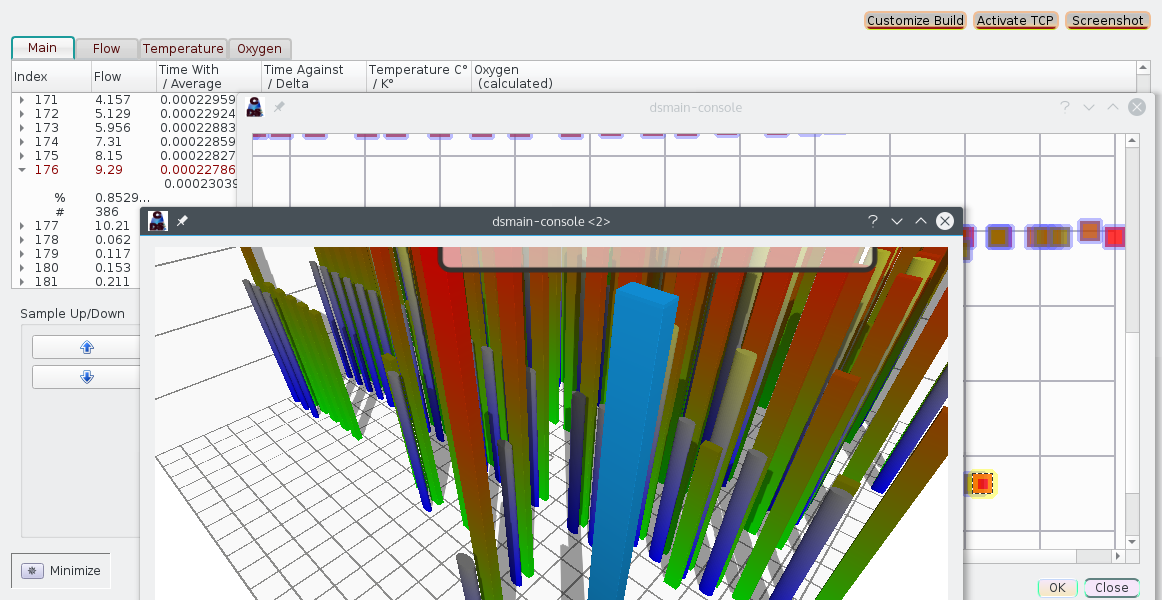
\includegraphics[scale=1]{texs/coord.png}}
            
  \node [text width=9.6cm,align=justify,fill=logoCyan!20, draw=logoBlue, 
  draw opacity=0.5,line width=1mm, fill opacity=0.9]
   at (0.785,0.445){\textbf{Dataset Applications can use 2- and 3D 
   visualization as well as textual/tabular displays, employing Reactive 
   Programming techniques to coordinate multiple visible windows.  For example, 
   visual cues direct attention to selected samples represented via 
   expanded rows (\circled{1}), color-highlighted 2D regions (\circled{2}), 
   and color-highlighted 3D bars (\circled{3}).  The main, 2D, 
   and 3D windows are functionally linked so that the same sample is 
   highlighted/expanded in each display window.}};
              
            \annotatedFigureBox{0.02,0.63}{0.057,0.74}{1}{0.057,0.74}%
            \annotatedFigureBox{0.825,0.16}{0.86,0.23}{2}{0.856,0.24}%            
            \annotatedFigureBox{0.55,0.42}{0.55,0.48}{3}{0.55,0.48}            
            
      %      \annotatedFigureBox{0.222,0.284}{0.3743,0.4934}{B}{0.3743,0.4934}%tr
      %      \annotatedFigureBox{0.555,0.784}{0.6815,0.874}{C}{0.555,0.784}%bl
      %      \annotatedFigureBox{0.557,0.322}{0.8985,0.5269}{D}{0.8985,0.5269}%tr
  

  
        \end{annotatedFigure}

   %     \caption{Expanded Sample (A)}
    %    \label{fig:teaser}

    \end{figure}

\end{frame}

